\subsection{Comments Upon Validity of Area Transformed Data}

As described in Subsection 4.1, the area fraction transformed ($\alpha$) was calculated for each optical frame simply as the average intensity of that frame.  The entire $\alpha$ curve for the sample was subsequently rescaled.  After this analysis was complete, however, it was observed that several of the videos comtain a faint lighting gradient, which may have negatively impacted the accuracy of the calculation.  Specifically, if the sample were improperly illuminated such that the crystalline regions received more or less light on average, then this would produce a systematic error in the results $\alpha$-curves.  Such a scenario becomes progressively more likely as the annealing temperature is lowered and the crystalline phase nucleates in a less-distributed manner.

A different analysis pipeline that addresses the issue would be to binarize and adaptively threshold each frame, thereby counting the fraction of pixels deemed ``bright enough'' to be crystalline based on local lighting conditions.  This, however, has the disadvantage of being sensitive to a dirtied optical lens; care would need to be taken to ignore pixels occluded by dirt or dust on the microscope. 

\subsection{Comments Upon Accuracy of Grain-Counting Algorithm}

Perhaps the most unsound decision made in this analysis was to avoid quantifying inaccuracies in the grain-counting algorithm of Subsection 4.2.  As shown in Figure \ref{fig:miscount}, the algorithm produces miscounts if it fails to find a local maximum for a given grain.  A more rigorous approach, such as that taken in Reference \cite{campbell:2018}, would involve aggressively overestimating the number of grains, after which a supplementary algorithm might be employed to merge adjacent watershed cells deemed similar enough to comprise a single grain.

The possibility of testing the algorithm against computer-generated training data was considered.  In this scenario, bright field and dark field images would be digitally generated for a variety of grain densities, then fed to the algorithm in order to quantify its standard error.  This error would then be translated to error in $\dot{N}/v$ and propagated through the remainder of the calculations.  The main obstacle to this analysis \textit{in silico} is that there is no way of guaranteeing that such artificial electron micrographs would possess qualities similar to real ones; the procedure would quantify the algorithm's error with respect to the sythetic data set only.

In this respect, the results of the grain-counting algorithm should only by viewed as a loose estimate, albeit with greator rigor and consistency than manual counting.

	\begin{figure}[h]
		\centering
		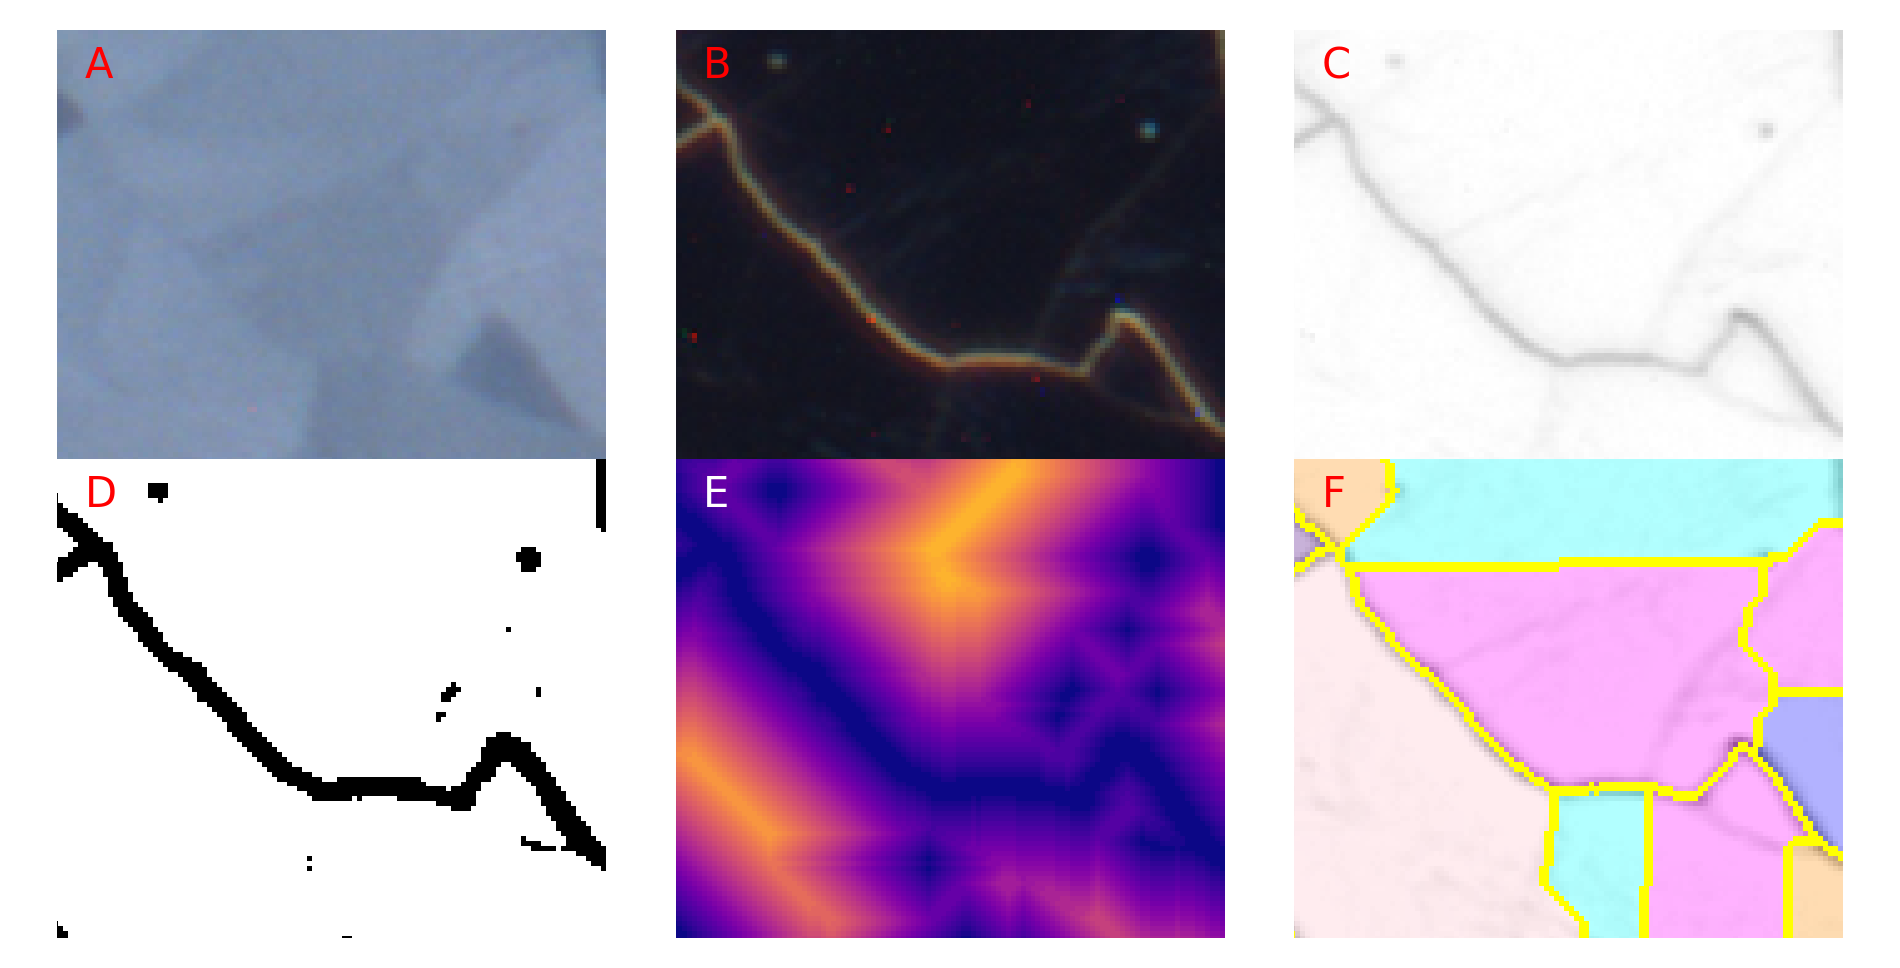
\includegraphics[width=1.0\linewidth]{miscount_10C.png}
		\caption{}
		\label{fig:miscount}
	\end{figure}

\subsection{Validity of Obtained Crystallization Parameters}

As evidenced by the graph in Figure \ref{fig:cluster_size}, the results of the parameter calculations of Subsection 4.3 do not truly yield an estimate for $g_{c \rightarrow a}$ and $i_c$, but rather a methodology for predicting them based on an estimate of $\gamma$.  From its lower limit of 2.683 atoms, the critical cluster size may be made arbitrarily large by changing the input $\gamma$, and a literature review yielded no methodology (beyond large-scale atomic simulations) for calculating the energy of the crystalline-amorphous interface.  These parameters should also be regarded with skepticism, given the assumption of a spherical nucleus with isotropic properties; in reality, Te manifests a trigonal crystal structure with a highly-anisotropic Wulff shape.  Refining the calculation to reflect these properties would likely require reengineering the Becker-Doering and JMAK results from the ground up.

Despite these reservations regarding the fundamental parameters of the crystalline-amorphous transformation, the Arrhenius laws for $\dot{N}$ and $v$ appear to fit the data moderately well, and as such may be used to predict the samples' annealing behavior.  The large standard errors of the prefactors in Table \ref{parameters_result} are a byproduct of fitting the data in $1/T$-ln coordinates; the actual coefficients of determination for the linear fit are $R^2_{\dot{N}} = 0.970$ and $R^2_v = 0.894$.  Most of the uncertainty appears to stem from the grain counts at 25 \textdegree{C} and 30 \textdegree{C}, which appear to be above and below the trend set by the other data, respectively.

